\chapter{Specifica dei casi d'uso}

\section{Introduzione}
In questo documento sono analizzati ed elencati gli attori ed i casi d'uso del sistema.
Scopo del documento è la dettagliata descrizione delle modalità di interazione tra le diverse entità presenti ed il sistema.
Ciò permetterà di mettere in evidenza eventuali conflitti tra i requisiti del sistema stesso.
Tale analisi e descrizione dei casi d'uso verrà presentata tramite grafici che seguono lo standard UML.

Nei casi in cui più attori possono accedere ad un determinato caso d’uso, ma uno
solo ha come compito quella operazione, non verranno elencati tutti gli attori
ma solo quello a cui quel caso appartiene.

Inoltre non verranno riportati tutti gli attori che hanno accesso ad un dato caso d'uso ma solo quello più generico.



\section{Elenco degli attori}
Gli attori che interagiscono con il portale sono elencati di seguito:
\begin{itemize}
	\item \newListItem{att:visitatore}{\formattaAtt}{Visitatore}
	\item \newListItem{att:utente}{\formattaAtt}{Utente}
	\item \newListItem{att:produttore}{\formattaAtt}{Produttore}
	\item \newListItem{att:redattore}{\formattaAtt}{Redattore}
	\item \newListItem{att:assistente}{\formattaAtt}{Assistente}
	\item \newListItem{att:moderatore}{\formattaAtt}{Moderatore}
	\item \newListItem{att:amministratore}{\formattaAtt}{Amministratore}
	\item \newListItem{att:cms}{\formattaAtt}{CMS}
\end{itemize}
La gerarchia degli attori è mostrata nel seguente diagramma UML:
\begin{center}
   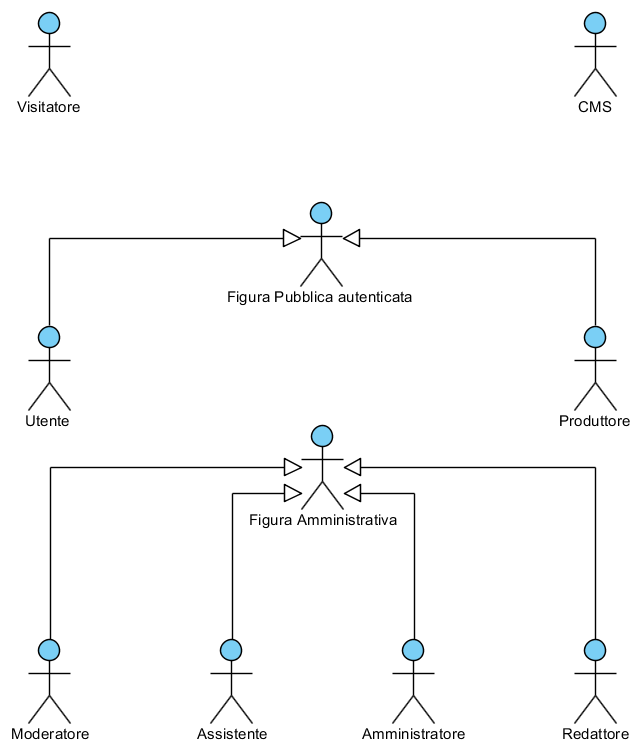
\includegraphics[width=\textwidth]{assets/visualParadigm/SchemaAttori}
\end{center}

\section{Specifica degli attori}
Gli attori che interagiscono con il portale sono descritti di seguito:
\attTab{att:visitatore}{-}{\glsdesc*{visitatore}}

\tabattvspace

\attTab{att:utente}{\getTitletodesc{att:visitatore}}{\glsdesc*{utente}}

\tabattvspace

\attTab{att:produttore}{\getTitletodesc{att:visitatore}}{\glsdesc*{produttore}}

\tabattvspace

\attTab{att:redattore}{\getTitletodesc{att:utente}}{\glsdesc*{redattore}}

\tabattvspace

\attTab{att:assistente}{\getTitletodesc{att:utente}}{\glsdesc*{assistente}}

\tabattvspace

\attTab{att:moderatore}{\getTitletodesc{att:utente}}{\glsdesc*{moderatore}}

\tabattvspace

\attTab{att:amministratore}{\getTitletodesc{att:utente}}{\glsdesc*{amministratore}}

\tabattvspace

\attTab{att:cms}{-}{\glsdesc*{cmsdef}}

\section{Identificativo dei casi d'uso} %(vengono usati per definire l'ID, non ha senso metterli dopo la struttura ID)
Di seguito è spiegato come interpretare l'identificativo dei casi d'uso:
\begin{center}
	\use{categoria}{caso}%{[sottoreq]}{[\dots]}
\end{center}

\noindent
Segue una descrizione di ogni campo utilizzato nell'identificatore:
\begin{itemize}
	\item La \campiIdReq{categoria} è una lettera utilizzata per raggruppare i casi d'uso con scopi simili.
	Le categorie sono le seguenti:
	\begin{enumerateIndLabel}{\textsf{\Alph*}}{\Alph*}
		\item Autenticazione. \label{pkg:autenticazione}
		\item Gestione iscrizioni. \label{pkg:iscrizione}
		\item Gestione vetrina. \label{pkg:vetrina} 
		\item Gestione notizie. \label{pkg:notizie}
		\item Gestione suggerimenti. \label{pkg:suggerimenti}
		\item Gestione account. \label{pkg:account}
		\item Gestione valutazioni. \label{pkg:gestionevalutazione}
		\item Gestione recensioni. \label{pkg:gestionerecensione}
		\item Interazione tra figure. \label{pkg:interazione}
		\item Gestione ticket. \label{pkg:gestioneticket}
		\item Ricerca contenuti. \label{pkg:ricerca}
		\item Gestione prodotti mancanti. \label{pkg:prodottimancanti}
		\item Visualizzazione contenuti pubblici. \label{pkg:visualizzazione}
	\end{enumerateIndLabel}

	\item Il campo \campiIdReq{caso} è un numero progressivo utilizzato per identificare in modo univoco un caso d'uso all'interno della sua categoria.
\end{itemize}

\section{Elenco dei casi d'uso}
Vengono di seguito elencati i casi d'uso:
\begin{itemize} 
	\setCatCU{\ref*{pkg:autenticazione}}%A
	\item \newListItem{cu:login}{\formattaCU}{Login}
	\item \newListItem{cu:logout}{\formattaCU}{Logout}

	\setCatCU{\ref*{pkg:iscrizione}}%B
	\item \newListItem{cu:iscrizionePortale}{\formattaCU}{Iscrizione tramite modulo del portale}
	\item \newListItem{cu:iscrizioneSocialVer}{\formattaCU}{Iscrizione tramite Social Network verificati}
	\item \newListItem{cu:iscrizioneSocialNotVer}{\formattaCU}{Iscrizione tramite Social Network non verificati}
	\item \newListItem{cu:iscrizioneApprovazione}{\formattaCU}{Iscrizione tramite approvazione}
	\item \newListItem{cu:approvazioneIscrizione}{\formattaCU}{Approvazione iscrizione}

	\setCatCU{\ref*{pkg:vetrina}}%C
	\item \newListItem{cu:personalizzaVetrinaInsDesc}{\formattaCU}{Inserimento descrizione}
	\item \newListItem{cu:personalizzaVetrinaInsImg}{\formattaCU}{Inserimento immagine}
	\item \newListItem{cu:personalizzaVetrinaInsProd}{\formattaCU}{Inserimento prodotto}
	\item \newListItem{cu:personalizzaVetrinaModProd}{\formattaCU}{Modifica prodotto}
	\item \newListItem{cu:statistichePrivateVetrina}{\formattaCU}{Visualizzazione statistiche private della vetrina}


	\setCatCU{\ref*{pkg:notizie}}%D
	\item \newListItem{cu:inserimentoNotizia}{\formattaCU}{Inserimento notizia}
	\item \newListItem{cu:modificaNotizia}{\formattaCU}{Modifica notizia}
	\item \newListItem{cu:rimozioneNotizia}{\formattaCU}{Rimozione notizia}

	\setCatCU{\ref*{pkg:suggerimenti}}%E
	\item \newListItem{cu:suggerimentoProdotti}{\formattaCU}{Suggerimento prodotti intelligente}
	\item \newListItem{cu:prodottiSimili}{\formattaCU}{Suggerimento prodotti simili}
	\item \newListItem{cu:notizieSimili}{\formattaCU}{Suggerimento notizie simili}

	\setCatCU{\ref*{pkg:account}}%F
	\item \newListItem{cu:accessoProfilo}{\formattaCU}{Accesso al proprio profilo}
	\item \newListItem{cu:accessoImpostazioni}{\formattaCU}{Accesso alle proprie impostazioni}
	\item \newListItem{cu:rimozioneAccountProprio}{\formattaCU}{Rimozione account proprio}

	\item \newListItem{cu:rimozioneAccountAltrui}{\formattaCU}{Rimozione account altrui}
	\item \newListItem{cu:aggiungiAccountAFigura}{\formattaCU}{Aggiungi funzionalità di una figura ad account}
	\item \newListItem{cu:rimuoviAccountDaFigura}{\formattaCU}{Rimuovi funzionalità di una figura da account}

	\setCatCU{\ref*{pkg:gestionevalutazione}}%G
	\item \newListItem{cu:inserisciValutazioneProdotto}{\formattaCU}{Inserimento valutazione}
	\item \newListItem{cu:modificaValutazioneProdotto}{\formattaCU}{Modifica valutazione}

	\setCatCU{\ref*{pkg:gestionerecensione}}%H
	\item \newListItem{cu:inserisciRecensioneProdotto}{\formattaCU}{Inserimento recensione}
	\item \newListItem{cu:modificaRecensioneProdotto}{\formattaCU}{Modifica recensione propria}
	\item \newListItem{cu:eliminaRecensioneProdotto}{\formattaCU}{Rimozione recensione propria}
	\item \newListItem{cu:commentoRecensione}{\formattaCU}{Commento a recensione}
	\item \newListItem{cu:giudizioRecensione}{\formattaCU}{Giudizio recensione}
	\item \newListItem{cu:segnalazioneContenutiInap}{\formattaCU}{Segnalazione contenuti inappropriati}
	\item \newListItem{cu:rimozioneContenutiInap}{\formattaCU}{Rimozione contenuti inappropriati}

	\setCatCU{\ref*{pkg:interazione}}%I
	\item \newListItem{cu:followAccount}{\formattaCU}{Follow account}
	\item \newListItem{cu:unFollowAccount}{\formattaCU}{Unfollow account}

	\setCatCU{\ref*{pkg:gestioneticket}}%J
	\item \newListItem{cu:ticketInvio}{\formattaCU}{Invio di un ticket}
	\item \newListItem{cu:ticketRisposta}{\formattaCU}{Risposta ad un ticket}
	\item \newListItem{cu:ticketChiudi}{\formattaCU}{Chiusura di un ticket}
	\item \newListItem{cu:ticketLettura}{\formattaCU}{Lettura di un ticket}

	\setCatCU{\ref*{pkg:ricerca}}%K
	\item \newListItem{cu:ricercaProdotto}{\formattaCU}{Ricerca prodotto}
	\item \newListItem{cu:ricercaProfilo}{\formattaCU}{Ricerca profilo}
	\item \newListItem{cu:ricercaNotizia}{\formattaCU}{Ricerca notizia}


	\setCatCU{\ref*{pkg:prodottimancanti}}%L
	\item \newListItem{cu:richiestaInsProdotto}{\formattaCU}{Richiesta inserimento prodotto a un produttore iscritto}
	\item \newListItem{cu:richiestaInsProduttore}{\formattaCU}{Richiesta inserimento prodotto e del suo produttore}

	\setCatCU{\ref*{pkg:visualizzazione}}%M
	\item \newListItem{cu:visualizzazioneVetrina}{\formattaCU}{Visualizzazione vetrina}
	\item \newListItem{cu:visualizzazioneStatistichePubVetrina}{\formattaCU}{Visualizzazione statische pubbliche vetrina}
	\item \newListItem{cu:visualizzazioneProdottiVetrina}{\formattaCU}{Visualizzazione prodotti esposti in vetrina}
	\item \newListItem{cu:visualizzazioneProdotto}{\formattaCU}{Visualizzazione prodotto}
	\item \newListItem{cu:visualizzazioneInfoProdotto}{\formattaCU}{Visualizzazione informazioni del prodotto}
	\item \newListItem{cu:visualizzazioneRecProdotto}{\formattaCU}{Visualizzazione recensioni associate al prodotto}
	\item \newListItem{cu:visualizzazioneStatProdotto}{\formattaCU}{Visualizzazione statistiche del prodotto}
	\item \newListItem{cu:visualizzazioneProfilo}{\formattaCU}{Visualizzazione profilo pubblico}
	\item \newListItem{cu:visualizzazioneInfoProfilo}{\formattaCU}{Visualizzazione informazioni di un profilo pubblico}
	\item \newListItem{cu:visualizzazioneStatProfilo}{\formattaCU}{Visualizzazione statistiche di un profilo pubblico}
	\item \newListItem{cu:visualizzazioneNotizie}{\formattaCU}{Visualizzazione notizie}
	\item \newListItem{cu:visualizzazioneAggF}{\formattaCU}{Visualizzazione aggiornamenti dai followed}
\end{itemize}	

%{id}{attori}{pre}{post}{flusso}
\section{Specifica dei casi d'uso}
\subsection{Autenticazione}
\begin{center}
   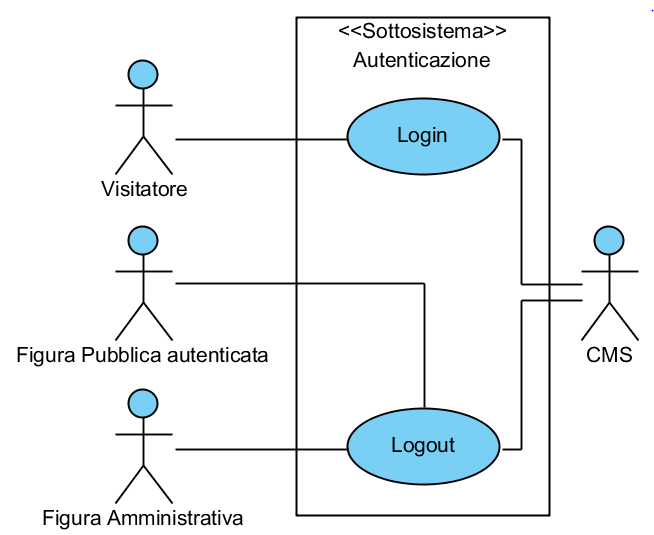
\includegraphics[width=\textwidth]{assets/visualParadigm/Autenticazione}
\end{center}
\cuTab{cu:login}{\getTitletodesc{att:visitatore}}{}{}{}
\cuTab{cu:logout}{\getTitletodesc{att:utente}, \getTitletodesc{att:produttore}, \getTitletodesc{att:redattore}, \getTitletodesc{att:assistente}, \getTitletodesc{att:moderatore}, \getTitletodesc{att:amministratore}}{}{}{}

\subsection{Gestione iscrizioni}
\begin{center}
   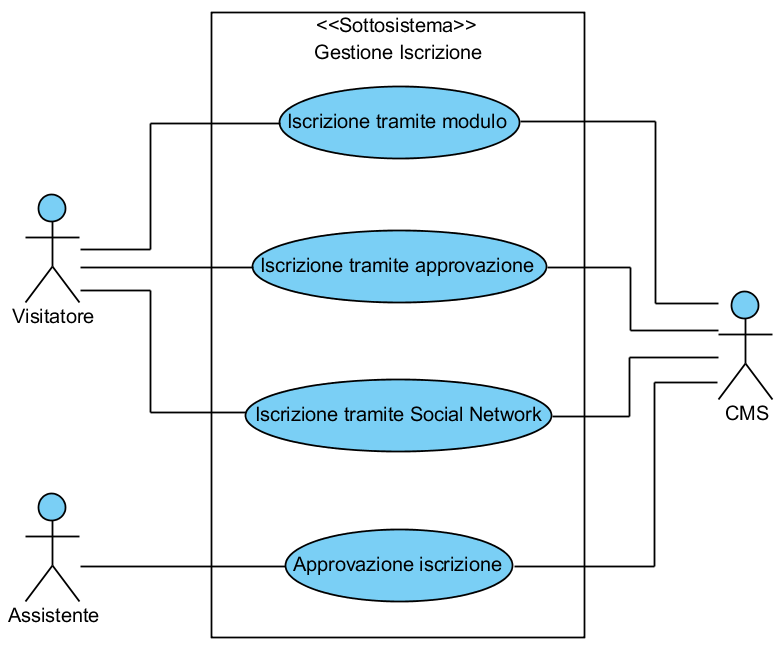
\includegraphics[width=\textwidth]{assets/visualParadigm/GestioneIscrizione}
\end{center}
\cuTab{cu:iscrizionePortale}{\getTitletodesc{att:visitatore}}{}{}{}
\cuTab{cu:iscrizioneSocialVer}{\getTitletodesc{att:visitatore}}{}{}{}
\cuTab{cu:iscrizioneSocialNotVer}{\getTitletodesc{att:visitatore}}{}{}{}
\cuTab{cu:iscrizioneApprovazione}{\getTitletodesc{att:visitatore}}{}{}{}
\cuTab{cu:approvazioneIscrizione}{\getTitletodesc{att:assistente}}{}{}{}

\subsection{Gestione vetrina}
\begin{center}
   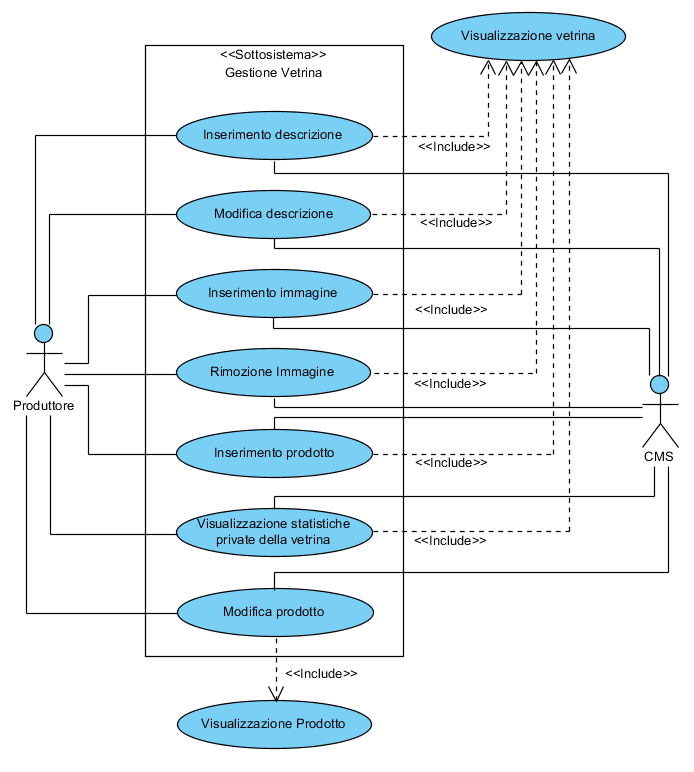
\includegraphics[width=\textwidth]{assets/visualParadigm/GestioneVentrina}
\end{center}
\cuTab{cu:personalizzaVetrinaInsDesc}{\getTitletodesc{att:produttore}}{}{}{}
\cuTab{cu:personalizzaVetrinaInsImg}{\getTitletodesc{att:produttore}}{}{}{}
\cuTab{cu:personalizzaVetrinaInsProd}{\getTitletodesc{att:produttore}}{}{}{}
\cuTab{cu:personalizzaVetrinaModProd}{\getTitletodesc{att:produttore}}{}{}{}
\cuTab{cu:statistichePrivateVetrina}{\getTitletodesc{att:produttore}}{}{}{}

\subsection{Gestione notizie}
\begin{center}
   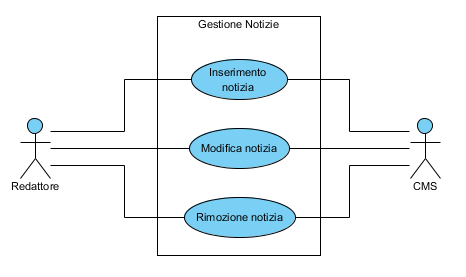
\includegraphics[width=\textwidth]{assets/visualParadigm/GestioneNotizie}
\end{center}
\cuTab{cu:inserimentoNotizia}{\getTitletodesc{att:redattore}}{}{}{}
\cuTab{cu:modificaNotizia}{\getTitletodesc{att:redattore}}{}{}{}
\cuTab{cu:rimozioneNotizia}{\getTitletodesc{att:redattore}}{}{}{}

\subsection{Gestione suggerimenti}
\begin{center}
   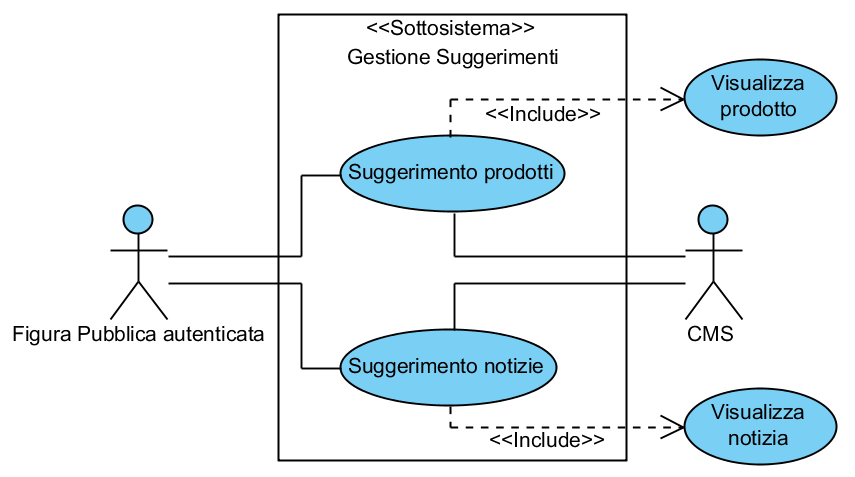
\includegraphics[width=\textwidth]{assets/visualParadigm/GestioneSuggerimenti}
\end{center}
\cuTab{cu:suggerimentoProdotti}{\getTitletodesc{att:utente}, \getTitletodesc{att:produttore}}{}{}{}
\cuTab{cu:prodottiSimili}{\getTitletodesc{att:utente}, \getTitletodesc{att:produttore}}{}{}{}
\cuTab{cu:notizieSimili}{\getTitletodesc{att:utente}, \getTitletodesc{att:produttore}}{}{}{}

\subsection{Gestione account}
\begin{center}
   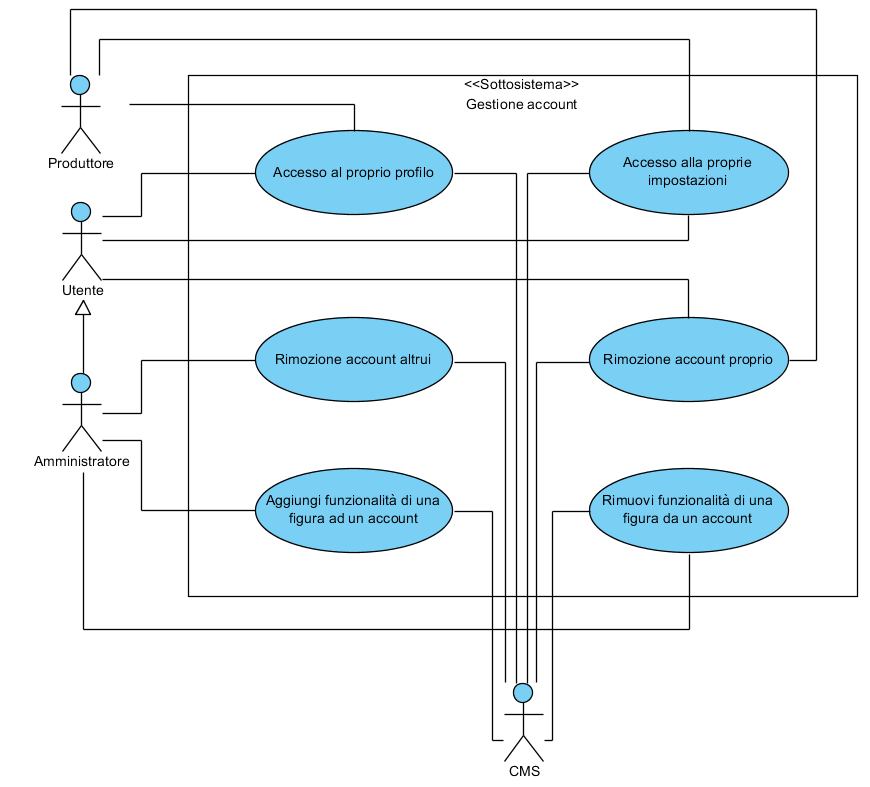
\includegraphics[width=\textwidth]{assets/visualParadigm/GestioneAccount}
\end{center}
\cuTab{cu:accessoProfilo}{\getTitletodesc{att:utente}, \getTitletodesc{att:produttore}}{}{}{}
\cuTab{cu:accessoImpostazioni}{\getTitletodesc{att:utente}, \getTitletodesc{att:produttore}}{}{}{}
\cuTab{cu:rimozioneAccountProprio}{\getTitletodesc{att:utente}, \getTitletodesc{att:produttore}}{}{}{}
\cuTab{cu:rimozioneAccountAltrui}{\getTitletodesc{att:amministratore}}{}{}{}
\cuTab{cu:aggiungiAccountAFigura}{\getTitletodesc{att:amministratore}}{}{}{}
\cuTab{cu:rimuoviAccountDaFigura}{\getTitletodesc{att:amministratore}}{}{}{}

\subsection{Gestione valutazioni}
\begin{center}
   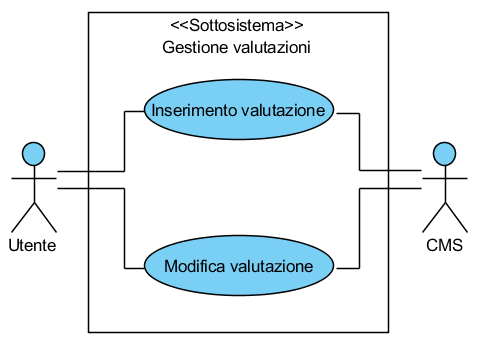
\includegraphics[width=\textwidth]{assets/visualParadigm/GestioneValutazioni}
\end{center}
\cuTab{cu:inserisciValutazioneProdotto}{\getTitletodesc{att:utente}}{}{}{}
\cuTab{cu:modificaValutazioneProdotto}{\getTitletodesc{att:utente}}{}{}{}

\subsection{Gestione recensioni}
\begin{center}
   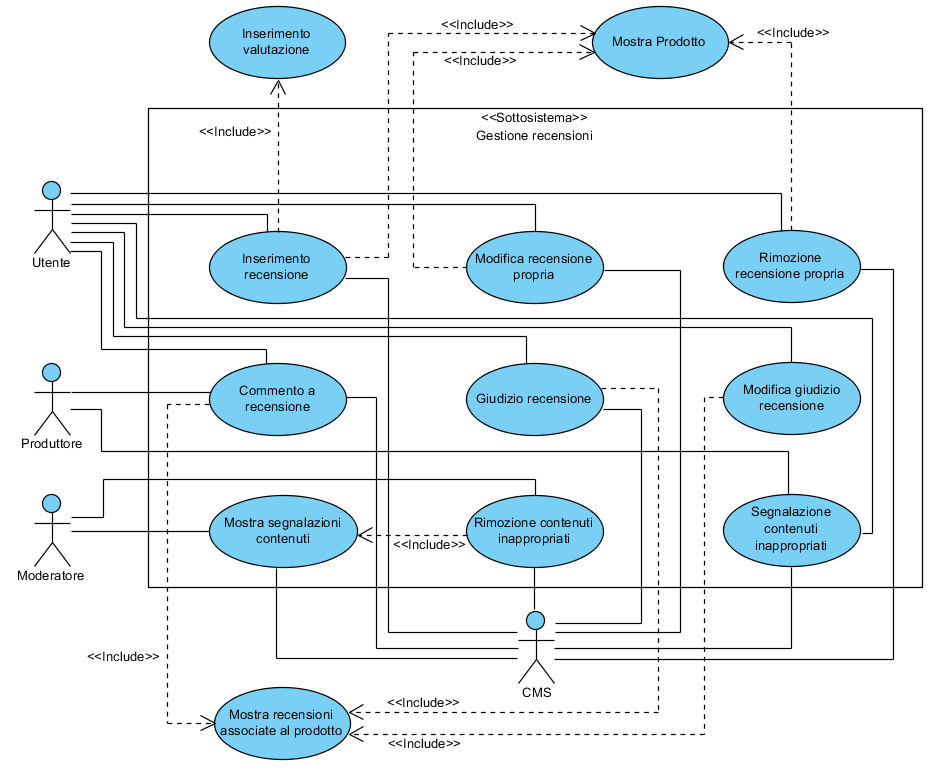
\includegraphics[width=\textwidth]{assets/visualParadigm/GestioneRecensioni}
\end{center}
\cuTab{cu:inserisciRecensioneProdotto}{\getTitletodesc{att:utente}}{}{}{}
\cuTab{cu:modificaRecensioneProdotto}{\getTitletodesc{att:utente}}{}{}{}
\cuTab{cu:eliminaRecensioneProdotto}{\getTitletodesc{att:utente}}{}{}{}
\cuTab{cu:commentoRecensione}{\getTitletodesc{att:utente}, \getTitletodesc{att:produttore}}{}{}{}
\cuTab{cu:giudizioRecensione}{\getTitletodesc{att:utente}}{}{}{}
\cuTab{cu:segnalazioneContenutiInap}{\getTitletodesc{att:utente}, \getTitletodesc{att:produttore}}{}{}{}
\cuTab{cu:rimozioneContenutiInap}{\getTitletodesc{att:moderatore}}{}{}{}

\subsection{Interazione tra figure}
\begin{center}
   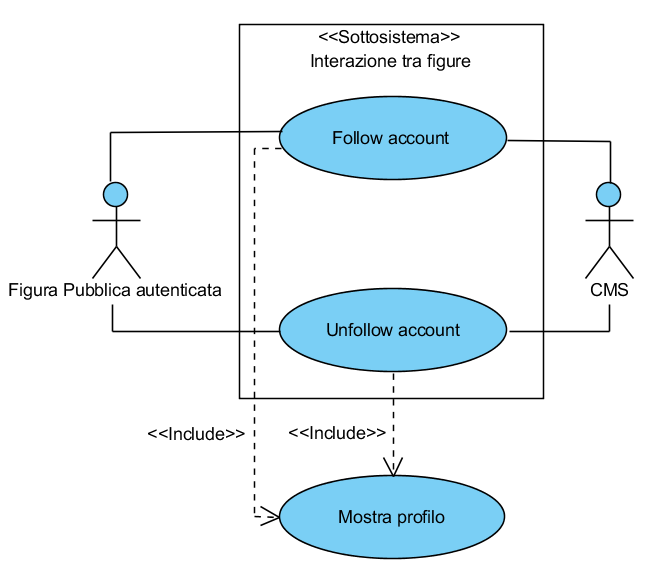
\includegraphics[width=\textwidth]{assets/visualParadigm/InterazioneTraFigure}
\end{center}
\cuTab{cu:followAccount}{\getTitletodesc{att:utente}, \getTitletodesc{att:produttore}}{}{}{}
\cuTab{cu:unFollowAccount}{\getTitletodesc{att:utente}, \getTitletodesc{att:produttore}}{}{}{}

\subsection{Gestione ticket}
\begin{center}
   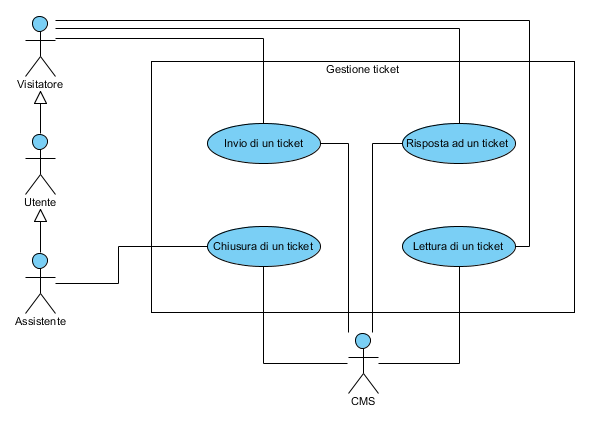
\includegraphics[width=\textwidth]{assets/visualParadigm/GestioneTicket}
\end{center}
\cuTab{cu:ticketInvio}{\getTitletodesc{att:visitatore}, \getTitletodesc{att:utente}, \getTitletodesc{att:produttore}}{}{}{}
\cuTab{cu:ticketRisposta}{\getTitletodesc{att:visitatore}, \getTitletodesc{att:utente}, \getTitletodesc{att:produttore}, \getTitletodesc{att:assistente}}}{}{}{}
\cuTab{cu:ticketChiudi}{\getTitletodesc{att:assistente}}{}{}{}
\cuTab{cu:ticketLettura}{\getTitletodesc{att:visitatore}, \getTitletodesc{att:utente}, \getTitletodesc{att:produttore},\getTitletodesc{att:assistente}}{}{}{}

\subsection{Ricerca contenuti}
\begin{center}
   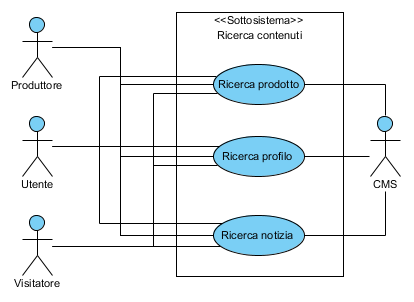
\includegraphics[width=\textwidth]{assets/visualParadigm/RicercaContenuti}
\end{center}
\cuTab{cu:ricercaProdotto}{\getTitletodesc{att:visitatore}, \getTitletodesc{att:utente}, \getTitletodesc{att:produttore}}{}{}{}
\cuTab{cu:ricercaProfilo}{\getTitletodesc{att:visitatore}, \getTitletodesc{att:utente}, \getTitletodesc{att:produttore}}{}{}{}
\cuTab{cu:ricercaNotizia}{\getTitletodesc{att:visitatore}, \getTitletodesc{att:utente}, \getTitletodesc{att:produttore}}{}{}{}

\subsection{Gestione prodotti mancanti}
\begin{center}
   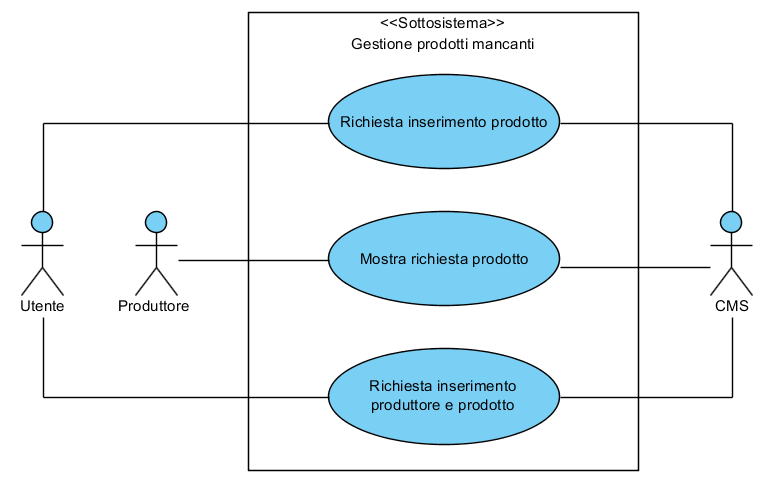
\includegraphics[width=\textwidth]{assets/visualParadigm/GestioneProdottiMancanti}
\end{center}
\cuTab{cu:richiestaInsProdotto}{\getTitletodesc{att:utente}}{}{}{}
\cuTab{cu:richiestaInsProduttore}{\getTitletodesc{att:utente}}{}{}{}

\subsection{Visualizzazione contenuti pubblici}
\begin{center}
   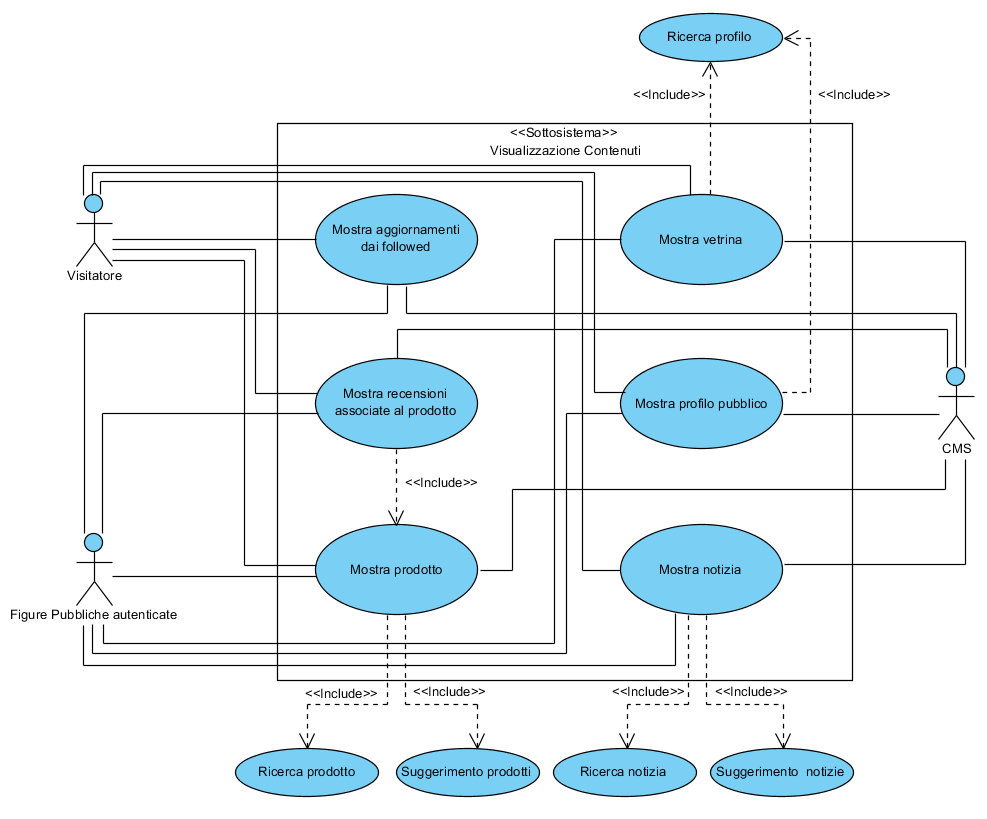
\includegraphics[width=\textwidth]{assets/visualParadigm/Visualizzazione}
\end{center}
\cuTab{cu:visualizzazioneVetrina}{\getTitletodesc{att:visitatore}, \getTitletodesc{att:utente}, \getTitletodesc{att:produttore}}{}{}{}
\cuTab{cu:visualizzazioneStatistichePubVetrina}{\getTitletodesc{att:visitatore}, \getTitletodesc{att:utente}, \getTitletodesc{att:produttore}}{}{}{}
\cuTab{cu:visualizzazioneProdottiVetrina}{\getTitletodesc{att:visitatore}, \getTitletodesc{att:utente}, \getTitletodesc{att:produttore}}{}{}{}
\cuTab{cu:visualizzazioneProdotto}{\getTitletodesc{att:visitatore}, \getTitletodesc{att:utente}, \getTitletodesc{att:produttore}}{}{}{}
\cuTab{cu:visualizzazioneInfoProdotto}{\getTitletodesc{att:visitatore}, \getTitletodesc{att:utente}, \getTitletodesc{att:produttore}}{}{}{}
\cuTab{cu:visualizzazioneRecProdotto}{\getTitletodesc{att:visitatore}, \getTitletodesc{att:utente}, \getTitletodesc{att:produttore}}{}{}{}
\cuTab{cu:visualizzazioneStatProdotto}{\getTitletodesc{att:visitatore}, \getTitletodesc{att:utente}, \getTitletodesc{att:produttore}}{}{}{}
\cuTab{cu:visualizzazioneProfilo}{\getTitletodesc{att:visitatore}, \getTitletodesc{att:utente}, \getTitletodesc{att:produttore}}{}{}{}
\cuTab{cu:visualizzazioneInfoProfilo}{\getTitletodesc{att:visitatore}, \getTitletodesc{att:utente}, \getTitletodesc{att:produttore}}{}{}{}
\cuTab{cu:visualizzazioneStatProfilo}{\getTitletodesc{att:visitatore}, \getTitletodesc{att:utente}, \getTitletodesc{att:produttore}}{}{}{}
\cuTab{cu:visualizzazioneNotizie}{\getTitletodesc{att:visitatore}, \getTitletodesc{att:utente}, \getTitletodesc{att:produttore}}{}{}{}
\cuTab{cu:visualizzazioneAggF}{\getTitletodesc{att:utente}, \getTitletodesc{att:produttore}}{}{}{}





































%Struttura dei casi d'uso (ID) T_T
%Esempi:
%Lumiere -> Ogni caso `e identificato da una stringa del tipo CU.entit`a.sottoentit`a.caso.
%Airbnb.it -> package = PKG_<numero package>_<numero_sottopackage> | caso d'uso = UC_<numero package>_<numero caso d’uso> | attore = ATT_<num. Attore generico>_<num. Attore specifico>

%A me la struttura a package piace, possiamo racchiudere molti casi d'uso in categorie così.

%Scopiazzerei il grafico di Airbnb.it a pagina 9, utilizzando quella figura per descrivere il sistema a grandi linee, con i package. Mostrata questa, procederei con l'analisi
%dei package uno ad uno e quindi dei singoli casi d'uso.
%Per ogni caso d'uso, entrambi gli esempi fanno la descrizione stile Basi 2 con precondizioni e postcondizioni (oltre che attori coinvolti, nome, descrizione e flusso).
%A me piace


